\documentclass[onecolumn, draftclsnofoot,10pt, compsoc]{IEEEtran}
\usepackage{graphicx}
\usepackage{url}
\usepackage{setspace}
\usepackage{float}
\usepackage{cite}

\usepackage{geometry}
\geometry{textheight=9.5in, textwidth=7in}

% 1. Fill in these details
\def \CapstoneTeamName{Education Simulations}
\def \CapstoneTeamNumber{53}
\def \GroupMemberOne{Cameron Friel}
\def \GroupMemberTwo{Kelli Ann Ulep}
\def \GroupMemberThree{Samuel Wilson}
\def \CapstoneProjectName{Interactive 2D simulations to support Inquiry-Based Learning in Mechanical Engineering}
\def \CapstoneSponsorCompany{Oregon State University, School of Chemical, Biological, and Environmental Engineering}
\def \CapstoneSponsorPersonOne{Milo Koretsky}
\def \CapstoneSponsorPersonTwo{Tom Ekstedt}


% 2. Uncomment the appropriate line below so that the document type works
\def \DocType{		%Problem Statement
				%Requirements Document
				%Technology Review
				Design Document
				%Progress Report
				}
			
\newcommand{\NameSigPair}[1]{\par
\makebox[2.75in][r]{#1} \hfil 	\makebox[3.25in]{\makebox[2.25in]{\hrulefill} \hfill		\makebox[.75in]{\hrulefill}}
\par\vspace{-12pt} \textit{\tiny\noindent
\makebox[2.75in]{} \hfil		\makebox[3.25in]{\makebox[2.25in][r]{Signature} \hfill	\makebox[.75in][r]{Date}}}}
% 3. If the document is not to be signed, uncomment the RENEWcommand below
%\renewcommand{\NameSigPair}[1]{#1}

%%%%%%%%%%%%%%%%%%%%%%%%%%%%%%%%%%%%%%%
\begin{document}
\begin{titlepage}
    \pagenumbering{gobble}
    \begin{singlespace}
    	%
\includegraphics[height=4cm]{coe_v_spot1}
        \hfill 
        % 4. If you have a logo, use this includegraphics command to put it on the coversheet.
        %\includegraphics[height=4cm]{CompanyLogo}   
        \par\vspace{.2in}
        \centering
        \scshape{
            \huge CS Capstone \DocType \par
            {\large\today}\par
            \vspace{.5in}
            \textbf{\Huge\CapstoneProjectName}\par
            \vfill
            {\large Prepared for}\par
            \Huge \CapstoneSponsorCompany\par
            \vspace{5pt}
            {\Large
                \NameSigPair{\CapstoneSponsorPersonOne}\par
                \NameSigPair{\CapstoneSponsorPersonTwo}\par
            }
            {\large Prepared by }\par
            Group\CapstoneTeamNumber\par
            % 5. comment out the line below this one if you do not wish to name your team
            \CapstoneTeamName\par 
            \vspace{5pt}
            {\Large
                \NameSigPair{\GroupMemberOne}\par
                \NameSigPair{\GroupMemberTwo}\par
                \NameSigPair{\GroupMemberThree}\par
            }
            \vspace{20pt}
        }
        \begin{abstract}
        % 6. Fill in your abstract    
This project involves solving the problem of some universities lacking resources to visually show physical and mechanical interactions for Mechanical Engineering concepts.
This project is built on the research that shows that students can achieve a better understanding of difficult concepts by learning through interactive simulated environments.
By implementing 2D simulations based on these concepts, students will be able to visually interpret the concepts in the course.
The goal of this document is to document the design for these 2D simulations, explaining the implementations of the features which shall be expected for this project.
        \end{abstract}     
    \end{singlespace}
\end{titlepage}
\newpage
\pagenumbering{arabic}
\tableofcontents
% 7. uncomment this (if applicable). Consider adding a page break.
%\listoffigures
%\listoftables
\clearpage

% 8. now you write!
\section{Overview}
This document contains an in depth description of the designs to be used in the 2D Simulations for Inquiry-Based Learning project. This document will go over the UI design layouts needed for the simulation web page, the implementation of webpage hosting, and the implementation of the animation. The components within each of these sections are also explained. 

\subsection{Scope}
Our product will consist of six variations of a two dimensional simulation based on mechanical engineering concepts in order to support inquiry based learning for mechanical engineering students. The simulations will be hosted on the Concept Warehouse website, which is a website that provides interactive learning opportunities for classrooms. While the simulation is running, real time mathematical feedback will be provided in the form of graphs or simply values in the simulation. There will be start, stop, and reset button within each simulation so that the student can explore the simulations as many times or at as many points as they need to. The students will also be able to modify specific parameters within the sixth variation of the simulation, such as mass, friction, and angles.

\subsection{Purpose}
The purpose of this document is to present the design specifications for the Interactive 2D Simulations to support Inquiry-Based Learning in Mechanical Engineering project. This document will expand on the technologies used to implement the project, which will include:

\begin{itemize}
  \item The process of serving the simulations to the student
  \item The Game Engine used to procure the simulations
  \item User Interface designs for the web page
  \item Data Visualization
  \item Software for creating the simulation assets
\end{itemize} 

\subsection{Intended Audience}
The intended audience for this document is primarily for developers that will be working on the project and need to be on boarded. In addition to this, the document is used as verification to the client's of the project, Milo Koretsky and Tom Ekstedt, to make sure that the design falls inline with the expectations they have provided.


\section{Glossary}
\begin{itemize}
  \item Concept Warehouse - A platform for engineering students to answer questions inside or outside of class.
  \item User Interface (UI) - The aspect of a program that the user interacts with directly through keyboard and mouse.
  \item Simulation - A digital and visual representation of a physics model.
  \item Object - A particular instance of a class, where the object can be a combination of variables, functions, and data structures.
  \item JavaScript - A core scripting language used in the web. It is used to create interactive elements within a web page.
  \item Chart.js - A lightweight JavaScript library for creating interactive graphs and that is free to use for the web.
  \item Open-source - Software code that has been made available for public use and manipulation.
  \item Inkscape - A free and open-source 2D vector graphics editor.
  \item Defold - A free, 2D game engine, used by professional game developers.
  \item Coefficient of Restitution - ratio of the final to initial relative velocity between two objects after collision. Values range from 0 to 1
  \item Bootstrap - A toolkit for designing web applications
  \item Mockup - A prototype providing the design and functionality of a system 
  \item Input Bindings - Project wide table specifying how input translates into actions in the script
\end{itemize} 

% I think that we should get rid of this section. - Cameron
%copied this from the example we looked at
%\section{Design Description}
%\subsection{Introduction}

%\subsection{Design Stakeholders}

%\subsection{Design Concerns}

%\subsection{Design Views}

%\subsection{Design Viewpoints}

%\subsection{Design Elements}

%\subsection{Design Rationale}

\subsection{Design Timeline}
\begin{itemize}
    \item Jan 7 - Jan 20: UI creation
    \item Jan 20 - Feb 20: Simulation creation
    \item Feb 20 - Mar 22: Graph Add-on and Bug Fixes
    \item Mar 22 - April 10: Clean Up and Stretch Goals
    \item April 10 - Expo: Expo Preparation
\end{itemize}
% general timeline 

%\subsection{Design Languages}


\section{Design Viewpoints}
%Example: http://user.ceng.metu.edu.tr/~e1819002/SDD.pdf

\subsection{Introduction}
The different components of the web page is the hosting information, game engine, user interface, graphs, and art software. The following section explains each of the components and the implementation design. 
%********************************************
% Hosting information
%********************************************
\subsection{Hosting}
The project will consist of several files that will be delivered to the client. The client will then upload these files to their own server to be distributed to students. The end product will simply be a simulation that can be displayed to students.
The simulation consists of 5 pendulum variation cases and an exploratory mode. The flow of the system is that the instructor dictates when students are able to view the simulation through Concept Warehouse. Then the server updates the content of the web page with a new case. The cases are shown in sequential order from 1 to 5. Exploratory mode, where users can modify parameters, is also unlocked by the instructor. 

\begin{figure}[H]
  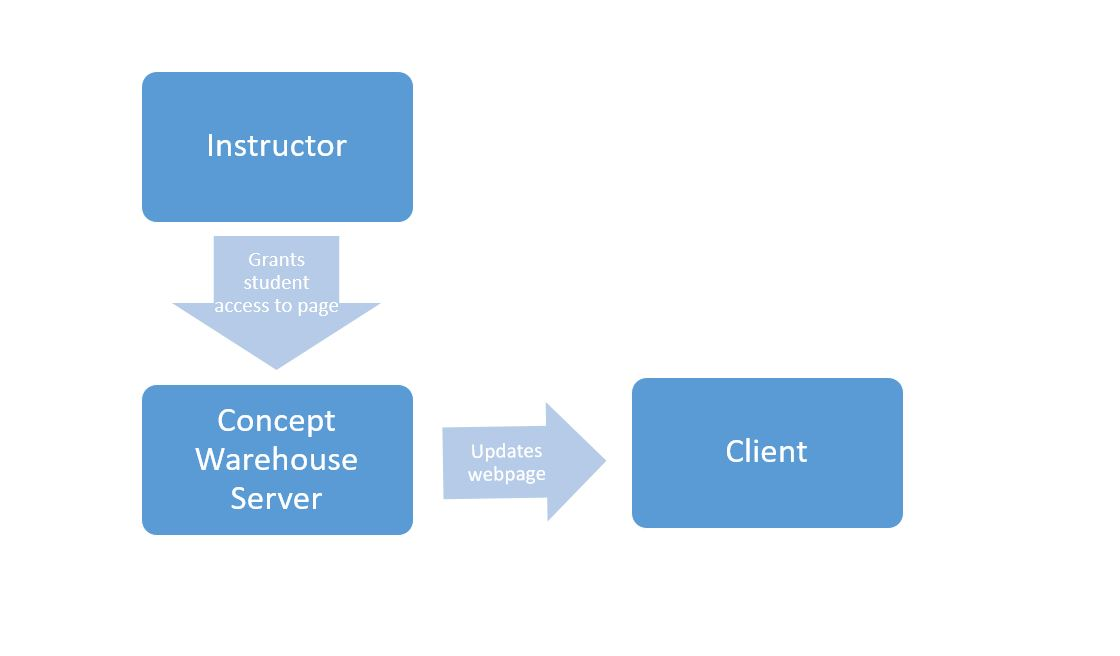
\includegraphics[width=6.5 in]{hosting_diagram.jpg}
  \caption{Hosting Diagram}
  \label{fig:host}
\end{figure}

%********************************************
% Game Engine
%********************************************
\subsection{Viewpoint: Game Engine}
%can add other subsections

\subsubsection{Design Concerns}
While game engines are useful for speeding up aspects of game creation, there is a risk that certain tools will not be usable for programs other than games. In this instance, the physics engine used may not work correctly with the projects simulations.

\subsubsection{Design Elements}
Game engines are programs which use an interface to allow easy creation and manipulation of UI and physics items. Certain functions that are common to game development, such as signals, are built-in. The main processes, which are unique to the game being created, are developed using scripts. These scripts are attached to individual elements of the game, though some can hold global variables. In the case of this project, the simulations being created are very similar to games. The team will use this similarity to their advantage by using game engines to quickly create physics simulations and UI.
%Design entities: class, interface, power type, data type, object, attribute, method, association class, template, and namespace.
%Design relationships: association, generalization, dependency, realization, implementation, instance of,composition, and aggregation.
%Design attributes: name, role name, visibility, cardinality, type, stereotype, redefinition, tagged value, parameter, and navigation efficiency.
%Design constraints: value constraints, relationships exclusivity constraints, navigability, generalization sets,multiplicity, derivation, changeability, initial value, qualifier, ordering, static, pre-condition, post-condition, and generalization set constraints.

%apparently u put whatever u need

\subsubsection{Function Attribute}
The game engine, Defold, will allow the team to quickly create multiple simulations of similar types. The ability to visually create the UI in real time will significantly increase production speeds, while maintaining the freedom of scripting.
\newline
\subsubsection{Pendulum Animation}
For the pendulum animation, the motion will be based on the following equation:
\begin{equation}
    \theta'' = (-1 * g/L)*sin(\theta)
\end{equation}
 where g = gravity, L = pendulum arm length, $\theta$ = angle in deg \newline
The angular acceleration of the pendulum is a constant of gravity divided by the length of the pendulum arm, multiplied by the sine of an angle. The velocity and position is changed over time.
%probably talk about friction/wind resistance
To account for air resistance or friction in the system, the angular velocity can be reduced by a constant each animation frame. 
\begin{equation}
   \theta' * k
\end{equation}
Where k is a constant between 0 and 1 where 0 is a stationary pendulum, and 1 is no air resistance. 
%https://www.khanacademy.org/computing/computer-programming/programming-natural-simulations/programming-oscillations/a/trig-and-forces-the-pendulum2
% don't know if they want "real" physics if they want damping but there's an even more complicated equation for that for box2d if they want. And can use forces to animate. 
%https://imranedu.wordpress.com/2015/01/07/how-to-simulate-realistic-air-friction-in-box2d-starling-version/

Defold includes a Box2D physics engine to simulate the physical interactions between two pendulums - for the cases that there are more than 1 weight in the pendulum system. The animation shall use the \textit{collision object} feature. 

%statement of what the entity does. The function attribute
%states the transformation applied by the entity to
%its inputs to produce the output. In the case of a data 
%entity, this attribute states the type of information
%stored or transmitted by the entity.

%\subsubsection{Relationship}



%********************************************
%  User interface
%********************************************
\subsection{Viewpoint: User Interface}
The User Interface is the gateway to connecting with the end user. It allows for interactivity with the simulation.
%can add other subsections

\subsubsection{Design Concerns}
A disorganized UI or a UI that is hard to understand can impede the student's learning. Even if the animation runs well in itself, if the web page it is placed in is hard to manipulate, it can take away from the animation. 

\subsubsection{Function Attribute: Normal Mode}
The user interface mockup of Case 1 is shown in Figure \ref{fig:case1_start} and Figure \ref{fig:case1_end}. Figure \ref{fig:case1_start} will be the initial screen shown. This will be the normal mode of case 1. Normal mode is applicable to all 5 of the variations of the impact pendulum scenario. 
The normal mode components with their description are as such:
\begin{itemize}
    \item Start/Pause Button - Starts the simulation or pauses it 
    \item Reset Button - Resets the simulation
    \item Graph of angle vs. time 
    \item Live measurement updates  - Updates the angle and height of each weight, velocity, and the time every 0.1 seconds of the simulation
    \item Starting measurements  - Length (m), weight (g), angle (degrees), height of weight off the ground (m), and coefficient of restitution 
\end{itemize}

The graph component design is explained in section 3.5. \newline


\begin{figure}[H]
  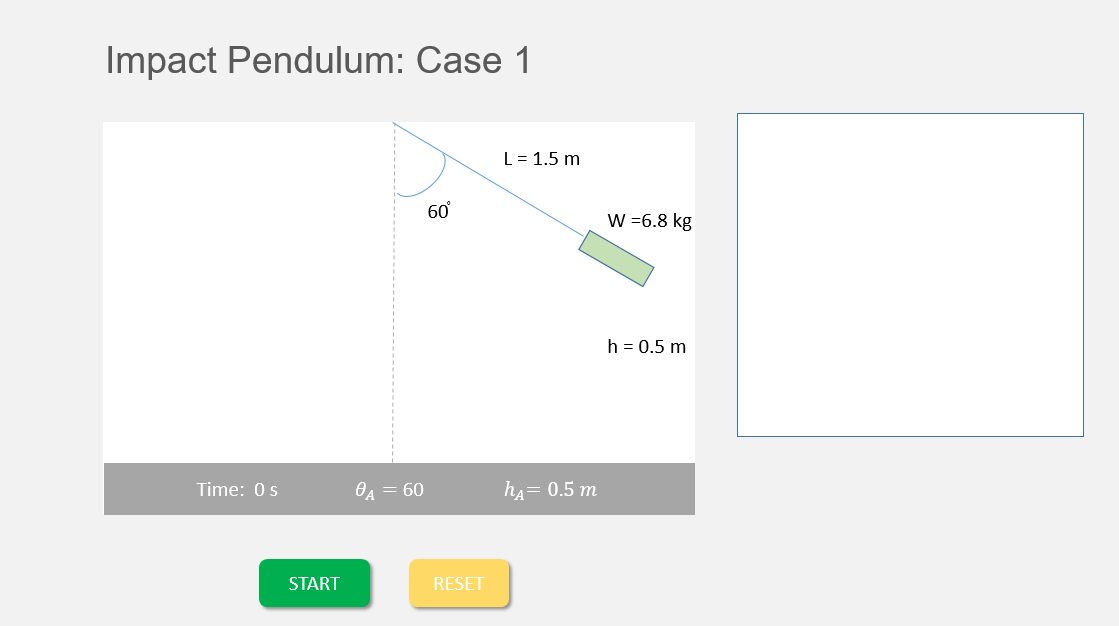
\includegraphics[width=5.5 in]{pendulum_case_1_1.png}
  \caption{Pendulum Case 1 - Before animation UI}
  \label{fig:case1_start}
\end{figure}
 
\begin{figure}[H]
  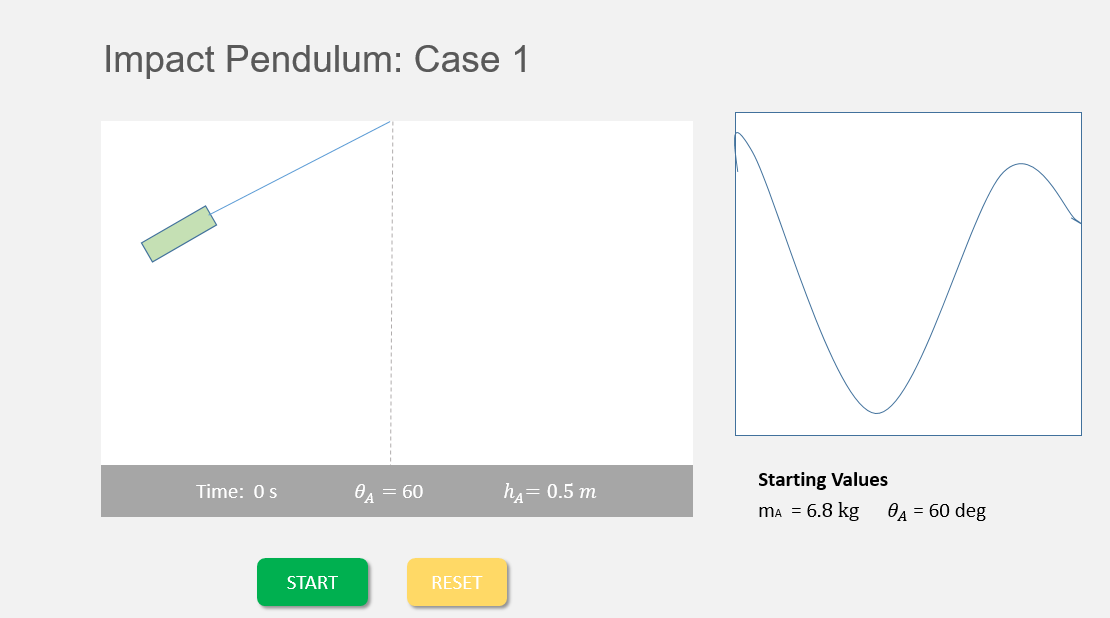
\includegraphics[width=5.5 in]{pendulum_case_1_2.png}
  \caption{Pendulum Case 1 - After animation completion UI}
  \label{fig:case1_end}
\end{figure}


\subsubsection{Function Attribute: Exploratory Mode}
The mockup of the Exploratory mode where the user can modify parameters is shown in Figure \ref{fig:explore_start} and Figure \ref{fig:explore_mid}. 
The exploratory mode components are
\begin{itemize}
  \item Start/Pause Button - Starts the simulation or pauses it 
    \item Reset Button - Resets the simulation
    \item Graph of angle vs. time 
    \item Live measurement updates  - Updates the angle and height of each weight, velocity, and the time every 0.1 seconds of the simulation
    \item Option to choose between 1 weight or 2 weights
    \item Starting parameter input sliders for the angle (degrees), length (m), weight (g), and coefficient of restitution.
\end{itemize}
\begin{figure}[H]
  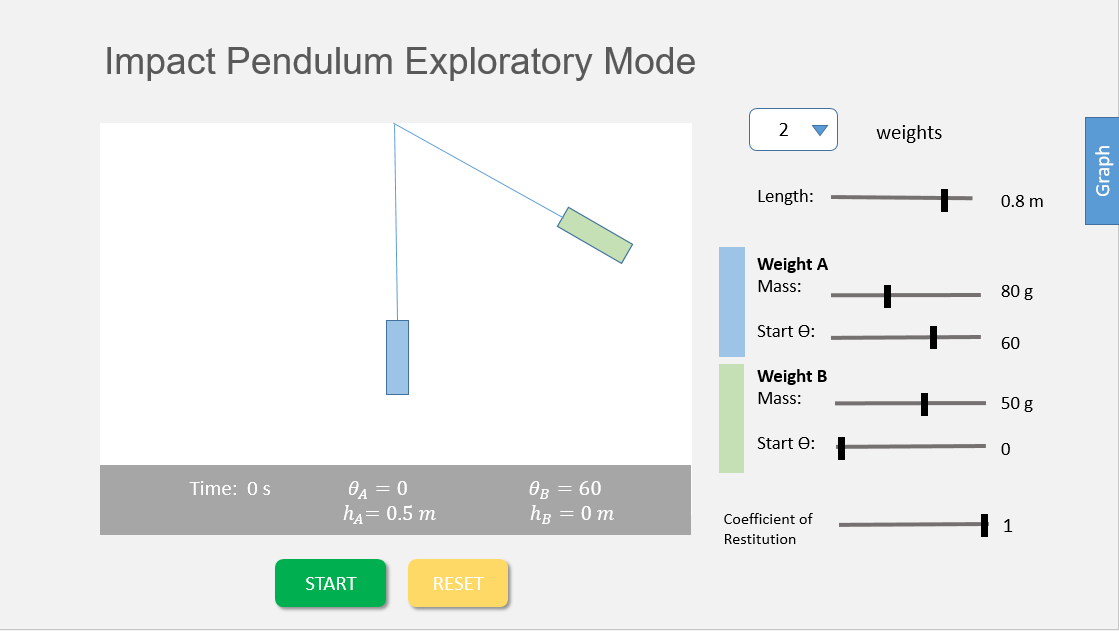
\includegraphics[width=\textwidth]{new_explore_s.png}
  \caption{Exploratory Mode Start Screen}
  \label{fig:explore_start}
\end{figure}
\begin{figure}[H]
  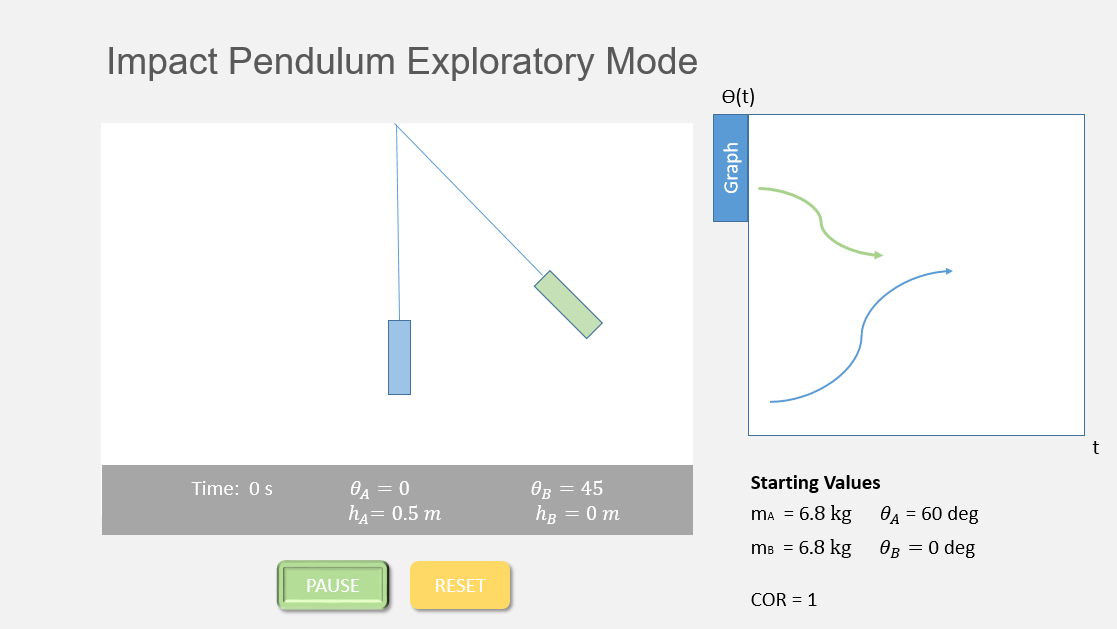
\includegraphics[width=\textwidth]{new_explore_mid.png}
  \caption{Exploratory Mode Mid Animation}
  \label{fig:explore_mid}
\end{figure}
%something about the input being limited 
%specific features of Defold 
%https://www.defold.com/manuals/input/
%https://rosettacode.org/wiki/Animate_a_pendulum#JavaScript
The game engine will construct the start/pause button, live measurement updates, and the input sliders and menu options. These components relate strongly to the animation.\newline
Defold has an input system to capture values from the mouse or keyboard and then dispatch the raw inputs as \textit{actions} to the script. The sliders, drop down menu, and the pendulum in the simulation can be told to listen for user input by sending the message "acquire\_input\_focus." The input bindings feature provides a table on how the input translates to the \textit{actions}. Then this the action is implemented on the object with the on\_input() function. 
%collision object 
The animation receives inputs from the input sliders and the drop down menu, so user input can be limited to reasonable measurements for the pendulum system. The values of length, mass, and starting angle will be passed into the pendulum motion formulas to affect the animation. The coefficient of restitution input will affect the pendulum game object's setting \textit{restitution} - affecting how the objects react after colliding (i.e. sticking together or not). Defold has a \textit{collision object} feature that has built in physical behavior and properties. 
\newline The graph of the weight's angle over time will replace the input sliders after starting the simulation. 
For styling of the UI, the Bootstrap library will be used in addition to the Defold canvas. Defold can build an application to run in a web page and can be provided with custom HTML and CSS. 
% End UI section **********************************

%********************************************
%  Graphing
%********************************************
\subsection{Viewpoint: Graphing}

\subsubsection{Design Concerns}
Graphs can be over stimulating if too much information is being presented to the viewer. Caution must be had when creating the graphs, so the layout is clear, and only important data points are being used.

\subsubsection{Design Elements}
 Graphs will be displayed to the screen with Chart.js, which is a lightweight JavaScript library that is free to use. Once the library is included with the script tag, a graph can be included by creating a Chart object with modifiable fields to build up your graph, such as, label for the graph's title, data for the graph's data to be graphed, and backgroundColor. After the object is made, it can be referenced to a canvas tag in order to be embedded within the web page.

\subsubsection{Function Attribute}
Graphs will be used within the UI for data visualization to provide the student with another resource to understand the interactions within the simulation.
% would a code example help here? https://www.chartjs.org/docs/latest/ 
% Any input appreciated! - Cameron


%********************************************
%  For the assets 
%********************************************
\subsection{Viewpoint: Art Software}

\subsubsection{Design Concerns}
The art involved in such dynamic programs is very important to conveying necessary information to the user. If the UI themes or graphics of a simulation are unclear, the user can miss interpret what is happening in the program, or lose interest in it due to poor quality. The color choices for the art themes of the interface are also extremely important, considering part of the user base will be blind to certain colors.

\subsubsection{Design Elements}
Using Inkscape, graphical representations for the elements of the simulations will be created to provide visible feedback to the user. These elements will be created in a way that makes it very clear to the user what they represent. The images provided in the User Interface section of this document give a good example of what these elements will look like.

\subsubsection{Function Attribute}
The art software chosen, Inkscape, will allow for the creation of simple and clear simulation graphics. Being open-source, Inkscape will also be available to everyone in the project team.

%\subsubsection{Relationship}

\subsection{Conclusion}
The core aspect of this project's development revolves around the use of the Defold game engine, which will be supported with the current UI designs, graphing scripts, and 2D images created with Inkscape.

\end{document}
